\section{Results}
\label{sec:results}
We present our multi-probe constraints on the cosmological parameters of the flat $\Lambda$CDM model in Fig.~\ref{fig:cosmology-params}, showing the marginalised posterior distributions for matter fluctuation amplitude parameter, $\sigma_8$, the matter density parameter, $\Omega_{\rm m}$, and the dimensionless Hubble parameter, $h$, where the BOSS galaxy clustering constraints (shown blue), break the $\sigma_8$-$\Omega_{\rm m}$ degeneracy in the KiDS-1000 cosmic shear constraints (shown pink), resulting in tight constraints on $\sigma_8$ in the combined \tttp analysis (shown red). 
Reporting the MAP values with PJ-HPD credible intervals for the parameters that we are most sensitive to, we find 
\eqa{
\sigma_8 &= \ksigmaeightval \\ \nonumber
\Omega_{\rm m} &= \kOmegamval \\ \nonumber
S_8 &= \kSeightval \, .
}
Our constraints can be compared to the marginalised posterior distributions from {\it Planck} (shown grey in Fig.~\ref{fig:cosmology-params}), finding consistency between the marginalised constraints on $\Omega_{\rm m}$ and $h$, but an offset in $\sigma_8$,  which we discuss in detail in Sect.~\ref{sec:planck_comp}.

Tabulated constraints for the full set of cosmological parameters are presented in Appendix~\ref{app:parameter-constraints}, quoting our fiducial MAP with PJ-HPD credible intervals along with the marginal posterior mode with M-HPD credible intervals. 
As discussed in \citet{joachimi/etal:inprep}, the marginal mode estimate is known to yield systematically low values of $S_8$ in mock data analyses.   This effect can be seen in Fig.~\ref{fig:S8comp} which compares the joint posterior constraints (solid) with the marginal posterior constraints (dashed).  

\begin{figure}
	\begin{center}
		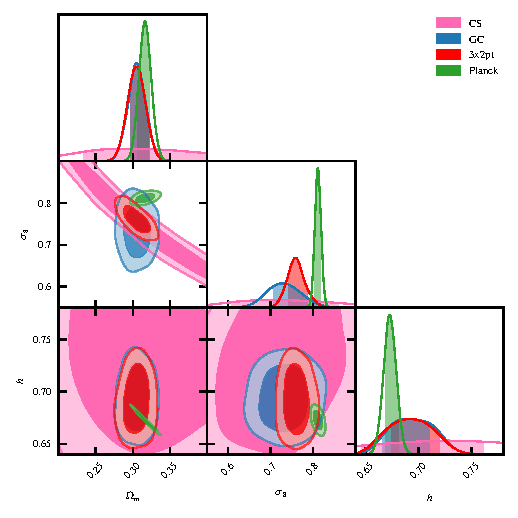
\includegraphics[width=\columnwidth]{Parameter_Plots/cosmology/omegam_sigma8_h_blind_C}
		\caption{Marginal multi-probe constraints on the flat $\Lambda$CDM cosmological model, for the matter fluctuation amplitude parameter, $\sigma_8$, the matter density parameter, $\Omega_{\rm m}$, and the dimensionless Hubble parameter, $h$.  The BOSS galaxy clustering constraints (blue), can be compared to the KiDS-1000 cosmic shear constraints (pink), the combined $3\times2{\rm pt}$ analysis (red), and CMB constraints from \citet[][grey]{planck/etal:2018}.}
		\label{fig:cosmology-params}
	\end{center}
\end{figure}

\begin{figure}
	\begin{center}
		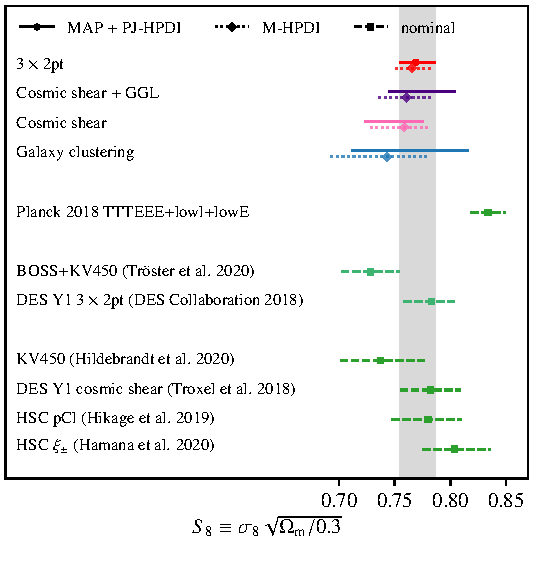
\includegraphics[width=\columnwidth]{Parameter_Plots/cosmology/S8_comparison_blindC}
		\caption{Constraints on the structure growth parameter $S_{8} = \sigma_8 \sqrt{\Omega_{\rm m}/0.3}$ for different probe combinations: $3\times2$pt, KiDS-1000 cosmic shear, BOSS galaxy clustering, cosmic shear with galaxy-galaxy lensing (GGL), and cosmic shear with galaxy clustering.   Our fiducial and preferred MAP with PJ-HPD credible interval (solid) can be compared to the standard, but shifted, marginal posterior mode with M-HPD credible intervals (dotted).    Our results can also be compared to weak lensing measurements from the literature, which typically quote the mean of the marginal posterior mode with tail credible intervals (dashed). 
		\label{fig:S8comp}}
	\end{center}
\end{figure}

We find good agreement between the different probe combinations and single-probe $S_8$ constraints, demonstrating internal consistency between the different cosmological probes, in Fig.~\ref{fig:S8comp}.  
As forecast by \citet{joachimi/etal:inprep}, the addition of the galaxy-galaxy lensing observable adds very little constraining power, with similar results found for the full \tttp analysis and the combined cosmic shear and clustering analysis. 
This is primarily a result of the significant full area of BOSS in comparison to the size of the BOSS-KiDS overlap region.   The lack of an accurate galaxy bias model on the deeply non-linear scales that weak lensing probes also prohibits the inclusion of large sections of our galaxy-galaxy lensing data vector, shown in Fig.~\ref{fig:Pgk}.  
The addition of the galaxy-galaxy lensing does, however, serve to moderately tighten constraints on the amplitude of the intrinsic alignment model $A_{\rm IA}$,  as seen in Fig.~\ref{fig:cosmology-params-all}. 

Fig.~\ref{fig:S8comp} also demonstrates the good agreement between our constraints and weak lensing results from the literature, comparing to cosmic shear-only results from the Hyper Suprime-Cam Strategic Programme \citep[HSC,][]{hikage/etal:2019,hamana/etal:2020}, DES Y1 \citep{troxel/etal:2018} and an earlier KiDS analysis \citep[KV450][]{hildebrandt/etal:2020}, in addition to the previous KV450-BOSS `$2\times2$pt' analysis of \citet{troester/etal:2020} and the DES Y1 \tttp analysis from \citet{abbott/etal:2018}.   We refer the reader to \citet{asgari/etal:inprep} for a discussion and comparison of different cosmic shear results.  In Sect.~\ref{sec:WL_comp} we present a more detailed comparison of our results with \tttp results in the literature.


\begin{figure*}
	\begin{center}
		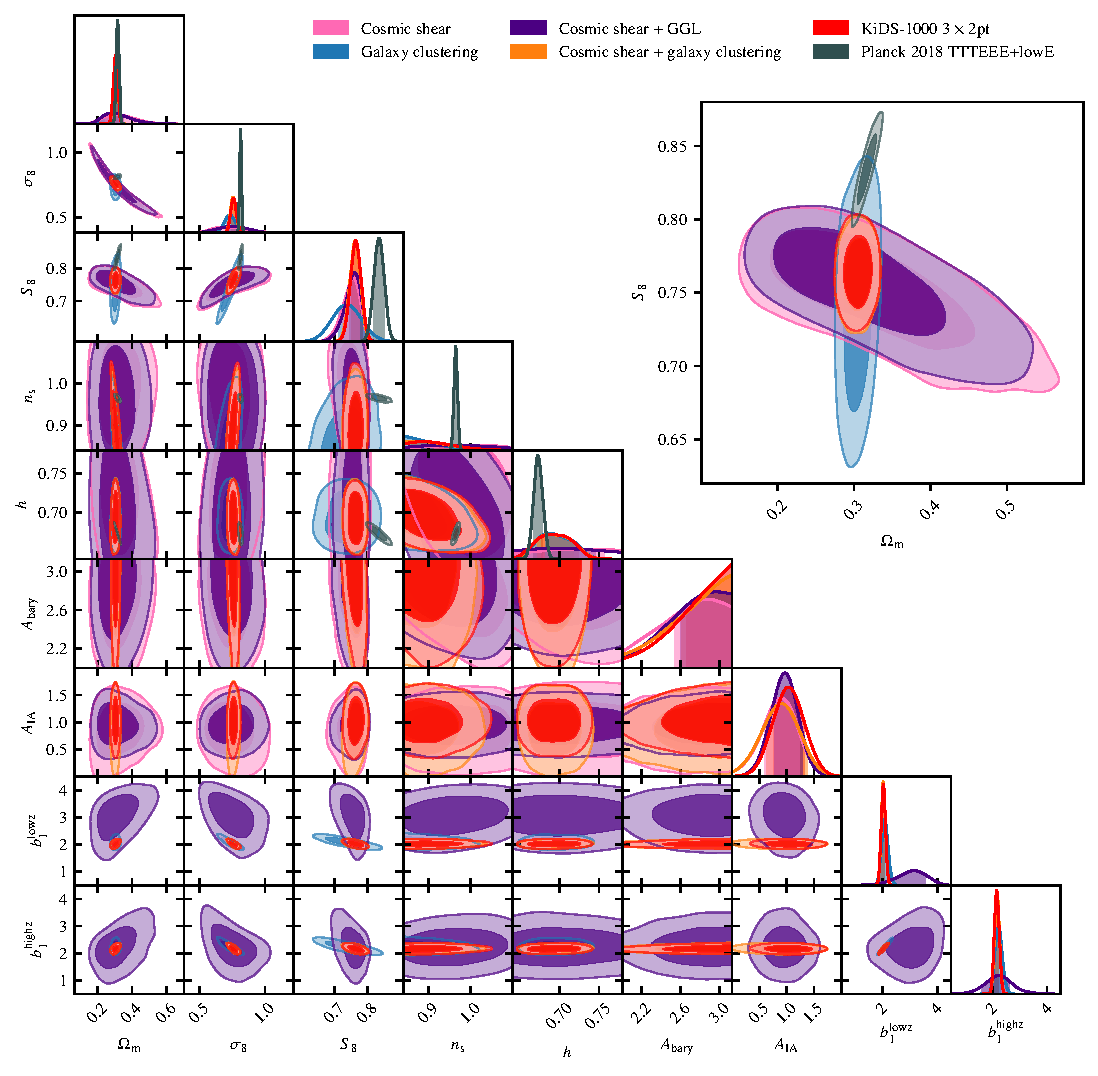
\includegraphics[width=\textwidth]{Parameter_Plots/cosmology/omegam_sigma8_s8_ns_h_a_baryon_a_ia_b1l_b1h_blind_C}
		\caption{Marginalised posterior distributions for an extended set of cosmological parameters covering the matter density parameter, $\Omega_{\rm m}$, the matter fluctuation amplitude parameter, $\sigma_8$, the structure growth parameter, $S_8$, the spectral index, $n_{\rm s}$, the dimensionless Hubble parameter, $h$, the baryon feedback amplitude parameter, $A_{\rm bary}$, the intrinsic alignment amplitude, $A_{\rm IA}$, and the linear bias parameters for the low and high BOSS redshift bins, $b_1$.   The KiDS-1000 cosmic shear results (pink), can be compared to the BOSS galaxy clustering results (blue), the combination of cosmic shear with BOSS and 2dFLenS galaxy-galaxy lensing (GGL, purple), and the full $3\times2$pt analysis (red).  The combination of cosmic shear with galaxy clustering (orange) is only distinguishable from the \tttp result in the $A_{\rm bary}$ and $A_{\rm IA}$ panels.  For parameters constrained by the CMB, we also include constraints from \citet[][grey]{planck/etal:2018}.}
		\label{fig:cosmology-params-all}
	\end{center}
\end{figure*}

Fig.~\ref{fig:cosmology-params-all} displays the marginal posterior distributions for an extended set of cosmological parameters.  
We find that the allowed range for the linear galaxy bias,  $b_1$, in each redshift bin (lower two rows), is almost halved with the addition of the weak lensing data. 
This constraint does not arise, however, from the sensitivity of the galaxy-galaxy lensing observable to galaxy bias (shown to be relatively weak in the purple cosmic shear + GGL contours). 
Instead, in this analysis, it is a result of the degeneracy breaking in the $\sigma_8$-$\Omega_{\rm m}$ plane, tightening constraints on $\sigma_8$ which, for galaxy clustering, is degenerate with galaxy bias. 
The improved constraints on galaxy bias do not, however, fold through to improved constraints on $h$, which the weak lensing data adds very little information to. 

\begin{table*}
	\begin{center}
		\caption{Goodness-of-fit of the flat $\Lambda$CDM cosmological model to each of the single and joint probe combinations with cosmic shear, galaxy clustering and galaxy-galaxy lensing (GGL).}
		\label{tab:goodness-of-fit}
\begin{tabular}{lcccccc}
    \toprule
    Probe             & $\chi^2_{\rm MAP}$  & Data DoF  & Model DoF                   & PTE  & Model DoF          & PTE    \\
                      &                     &           &\citep{joachimi/etal:inprep} &      & \citep{Raveri2019} & \\
    \midrule
	KiDS-1000 cosmic shear     & $152.1$ & $120$  &4.5 & 0.013 &3.0 & 0.016 \\
	BOSS galaxy clustering & $167.7$ & $168$  &-- & -- &10.6 & 0.272 \\
	Cosmic shear + GGL & $178.7$ & $142$  &8.7 & 0.005 &7.3 & 0.007 \\
	Cosmic shear + galaxy clustering & $319.9$ & $288$  &-- & -- &11.9 & 0.036 \\
	$3\times2$pt & $356.2$ & $310$  &-- & -- &12.5 & 0.011 \\

    \bottomrule
\end{tabular}
	\end{center}
	\tablefoot{We list the $\chi^2$ value at the maximum of the posterior, the number of degrees of freedom (DoF) of the data, the effective DoF of the model, and the probability to exceed (PTE) the measured $\chi^{2}$ value, assuming the total DoF are given by $\text{data DoF}-\text{model DoF}$. 
The effective DoF of the model are estimated following \citet{joachimi/etal:inprep} and \citet{Raveri2019}, accounting for the impact of priors and non-linear dependencies between the parameters. }
\end{table*}



For our primary cosmological parameter, $S_8$, our constraints are uninformed by our choice of priors.    This statement cannot be made for the other $\Lambda$CDM parameters, however, as shown in Fig.~\ref{fig:cosmology-params-all}.   The most informative prior that we have introduced to our \tttp analysis is on the spectral index, $n_{\rm s}$.  As noted by \citet{troester/etal:2020}, the BOSS galaxy clustering constraints favour a low value for $n_{\rm s}$, where they find $n_{\rm s} = 0.815 \pm 0.085$. 
From the \citet{troester/etal:2020} sensitivity analysis to the adopted maximum clustering scale we observe that this preference appears to be driven by the amplitude of the large scale clustering signal with $s > 100 \, h^{-1}\, {\rm Mpc}$.  We note that spurious excess power in this regime could plausibly arise from variations in the stellar density impacting the BOSS galaxy selection function \citep{ross/etal:2017}.  Our choice to impose a theoretically motivated informative prior for $n_{\rm s}$, as listed in Table~\ref{tab:priors}, helps to negate this potential systematic effect without degrading the overall goodness-of-fit to the galaxy clustering measurements.  Our prior choice is certainly no more informative than the $n_{\rm s}$ priors that are typically used in weak lensing and clustering analyses \citep[see for example][]{abbott/etal:2018,eBOSS/etal:2020}. 
We recognise, however, that this well-motivated prior choice acts to improve the BOSS-only error on $\Omega_{\rm m}$ by roughly a third, and decrease the BOSS-only best-fitting value for $\Omega_{\rm m}$ and $h$ by $\sim\! 0.5\,\sigma$ (see Fig.~\ref{fig:ns-prior}).  With $<10\%$ differences on the constraints on $S_8$ and $h$, however, and only a $\sim\! 0.1\,\sigma$ difference in the BOSS-only best-fitting value for $S_8$, which is consistent with the typical variation between different {\sc Multinest} analyses, we conclude that our prior choice does not impact on our primary $S_8$ constraints (see Appendix~\ref{app:priors}).   With the informative or uninformative $n_{\rm s}$ prior, our constraints on $h$ remain consistent with the Hubble parameter constraints from both \citet{planck/etal:2018} and \citet{riess/etal:2019}.

\begin{figure}
	\begin{center}
		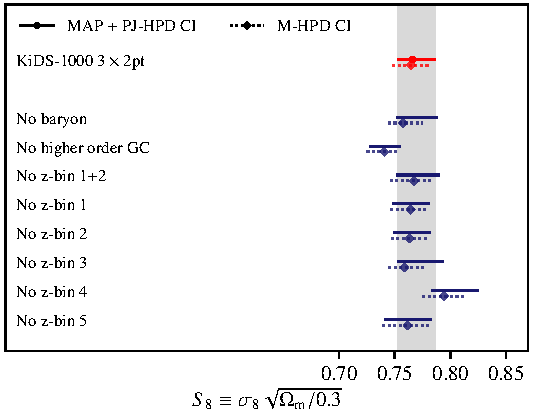
\includegraphics[width=\columnwidth]{Parameter_Plots/systematics/S8_comparison_blindC}
		\caption{\tttp constraints on $S_8$ for a series of sensitivity tests; when we ignore the impact of baryon feedback (the `No baryon' case), limit the analysis to a linear galaxy bias model (the `No higher order GC' case), and remove individual tomographic bins from our weak lensing observables.  
		\label{fig:S8comp_sensitivity}}
	\end{center}
\end{figure}

Fig.~\ref{fig:S8comp_sensitivity} illustrates the results of a series of sensitivity tests, where we explore how our \tttp constraints on $S_8$ change when: 
we ignore the impact of baryon feedback (the `No baryon' case) by fixing $A_{\rm bary}=3.13$, corresponding to the non-linear matter power spectrum for a dark-matter only cosmology; 
we limit the analysis to a linear galaxy bias model, setting all higher-order bias terms in Eq. (\ref{eq:pgg}) to zero, as well as restricting the redshift-space distortion model to a Gaussian velocity distribution; 
and we remove individual tomographic bins from our weak lensing observables. 
The systematic offset that arises from the use of a linear-bias model highlights the importance of accurate non-linear galaxy bias modelling in \tttp analyses.     
This series of tests is dissected further in Appendix~\ref{app:sensitivity}, and complements the detailed KiDS-1000 
internal consistency analysis of \citet[][appendix B]{asgari/etal:inprep}, 
which demonstrates that the change seen with the removal of tomographic bin 4 is fully consistent with expected statistical fluctuations.

Table~\ref{tab:goodness-of-fit} records the goodness-of-fit for each component in our \tttp analysis, where we report the $\chi^2$ value at the maximum posterior, $\chi^2_{\rm MAP}$ (see Sect.~\ref{sec:KCAP} for a discussion of our optimised MAP-finder).  
The effective number of degrees of freedom (DoF) does not equate to the standard difference between the total number of data points (Data DoF) and the total number of model parameters (20 in the case of our \tttp analysis), as a result of the adopted priors and the non-linear dependencies that exist between the model parameters.   For some probe combinations we calculate the effective number of degrees of freedom in the model (Model DoF), using the estimator described in section 6.3 of \citet{joachimi/etal:inprep}.    
As this approach is computationally expensive, however, we also estimate the Model DoF following \citet{Raveri2019}, recognising that, for the cases explored in \citet{joachimi/etal:inprep}, this approach results in a slightly lower model DoF.

We find that the goodness-of-fit is excellent for the BOSS galaxy clustering.  For all other cases, the goodness-of-fit is certainly acceptable\footnote{We define acceptable as the PTE $p \geq 0.001$, which corresponds to less than a $\sim\!3\,\sigma$ event.   \citet{abbott/etal:2018} define acceptable as $\chi^2/{\rm DoF} < 1.4$.  We meet both these requirements.}, with the probability to exceed the measured $\chi^2$ given by $p \gtrsim 0.01$.
We note that the cosmic shear analysis of \citet{asgari/etal:inprep} shows no significant changes in the inferred cosmological parameters when using different two-point statistics which exhibit an excellent goodness-of-fit.    As such, we could be subject to an unlucky noise fluctuation that particularly impacts the band power estimator in Eq. (\ref{eq:cl_cosmicshear}).  Cautiously inspecting Fig.~\ref{fig:Pkk}, as `$\chi$-by-eye' is particularly dangerous with correlated data points, we nevertheless note a handful of outlying points, for example the low $\ell$-scales in the fifth tomographic bin.   We also note that \citet{giblin/etal:inprep} document a significant but low-level PSF residual systematic in the KiDS-1000 fourth and fifth tomographic bins that was shown to reduce the overall goodness-of-fit in a cosmic shear analysis, but not bias the recovered cosmological parameters \citep[see the discussion in][]{amara/refregier:2008}.  Future work to remove these low-level residual distortions is therefore expected to further improve the goodness-of-fit.

\subsection{Comparison with weak lensing surveys}
\label{sec:WL_comp}
Our results are consistent with weak lensing constraints in the literature.   We limit our discussion in this section to published \tttp analyses, referring the reader to \citet{asgari/etal:inprep} who discuss how the KiDS-1000 cosmic shear results compare with other weak lensing surveys.   We note that direct comparisons of cosmological parameters should be approached with some caution, as the priors adopted by different surveys and analyses are often informative \citep[see section 6.1 in][]{joachimi/etal:inprep}.   Homogenising priors for cosmic shear analyses, for example, has been shown to lead to different conclusions when assessing inter-survey consistency \citep{chang/etal:2019, joudaki/etal:2020, asgari/etal:2020_KD}.   

\citet{abbott/etal:2018} present the first year \tttp DES analysis (DES Y1), finding $S_8=0.773^{+0.026}_{-0.020}$, where they report the marginal posterior maximum and the tail credible intervals.  
This is in excellent agreement with our equivalent result, differing by $0.3\,\sigma$, with the DES-Y1 error being 40\% larger than the KiDS-1000-BOSS \tttp results.  The inclusion of BOSS to our \tttp analysis results in tight constraints on $\Omega_{\rm m}$.  
This leads to joint KiDS-1000-BOSS constraints on $\sigma_8=0.760^{+0.021}_{-0.023}$ that are more than twice as constraining compared to the DES Y1-alone \tttp analysis which found $\sigma_8=0.817^{+0.045}_{-0.056}$, as shown in Fig.~\ref{fig:DES_KiDS_comp}. 
This comparison serves to highlight the additional power that can be extracted through the combination of spectroscopic and photometric surveys,  and the promising future for the planned overlap between the Dark Energy Spectroscopic Instrument survey \citep{DESI/etal:2016} and the 4-metre Multi-Object Spectroscopic Telescope \citep[4MOST,][]{richard/etal:2019},
with {\it Euclid} and the Vera C. Rubin Observatory Legacy Survey of Space and Time \citep{laureijs/etal:2011,lsst/etal:2009}, in addition to the nearer-term $\sim\!1400\,\mathrm{deg}^{2}$ of overlap between BOSS and HSC \citep{aihara/etal:2019}. 

\begin{figure}
	\begin{center}
		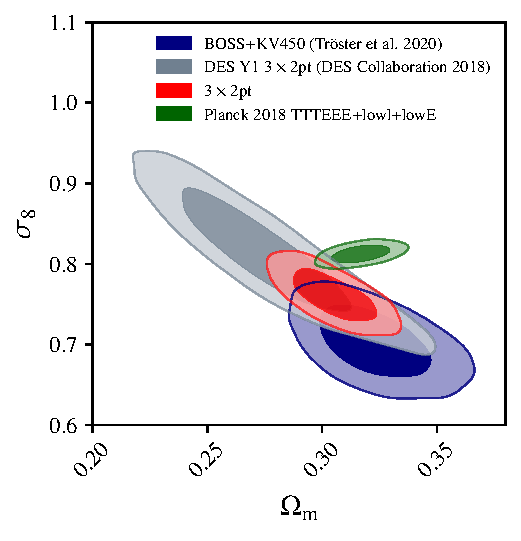
\includegraphics[width=\columnwidth]{Parameter_Plots/cosmology/omegam_sigma8_survey_comparison}
		\caption{Marginalised posterior distribution in the $\sigma_8$-$\Omega_{\rm m}$ plane, comparing the \tttp analyses from KiDS-1000 with BOSS and 2dFLenS, with the \tttp analysis from DES Y1 \citep{abbott/etal:2018}, and the CMB constraints from \citet{planck/etal:2018}.   The KiDS-1000 \tttp result can also be compared to our previous KV450-BOSS analysis from \citet{troester/etal:2020}. 
		\label{fig:DES_KiDS_comp}}
	\end{center}
\end{figure}

\citet{vanuitert/etal:2018} and \citet{joudaki/etal:2018} present \tttp analyses for the second KiDS weak lensing release (KiDS-450), finding, respectively, $S_8 = 0.800_{-0.027}^{+0.029}$ (KiDS with GAMA) and $S_8 = 0.742 \pm 0.035$ (KiDS with BOSS and 2dFLenS limited to the overlap region). 
Both results are consistent with our KiDS-1000 results, noting that the increase in our $S_8$ constraining power, by a factor of $\sim\! 2$ in this analysis, is driven by increases in both the KiDS survey area, and the analysed BOSS survey area.  

The impact of doubling the KiDS area can be seen by comparing to \citet{troester/etal:2020}, in Fig.~\ref{fig:DES_KiDS_comp}, who present a joint cosmic shear and galaxy clustering analysis of the KV450 KiDS release with the full BOSS area, finding $S_8 = 0.728 \pm 0.026$.   The $\sim\!40\%$ improvement in constraining power is consistent with expectations from the increased survey area, but a straightforward area-scaling comparison is inappropriate given that KiDS-1000 features improvements in the accuracy of the shear and photometric redshift calibrations, albeit at the expense of a decrease in the effective number density \citep[see][for details]{giblin/etal:inprep,hildebrandt/etal:inprep}.  

The offset in $S_8$ between the KiDS-1000-BOSS and KV450-BOSS $S_8$ constraints reflects a number of differences between the two analyses.  First, as the $S_8$ constraints from the \tttp analysis are primarily driven by KiDS (see Fig.~\ref{fig:cosmology-params-all}), we expect a reasonable statistical fluctuation in this parameter given the sampling variance arising from the significant increase in the KiDS survey area.  Using a simple model analysis in Appendix~\ref{app:expectedoffsets}, we conclude that we should expect differences, on average, of $|\Delta S_8| = 0.016$, and as such the increase that we find in $S_8$ between KV450 and KiDS-1000 is consistent with the expectation from simple statistical fluctuations.   BOSS primarily constrains $\Omega_{\rm m}$ which is impacted by the choice of prior on $n_{\rm s}$.  The wider $n_{\rm s}$ prior adopted in \citet{troester/etal:2020}, favours a slightly higher but less well-constrained value for $\Omega_{\rm m}$, leading to a slightly lower but less well-constrained value for $\sigma_8$, when combined with cosmic shear (see Appendix~\ref{app:priors}).   If we had also chosen an uninformative prior on $n_{\rm s}$ for our KiDS-1000-BOSS analysis, a decision that we cannot revise post unblinding, this would have likely served to exacerbate any tension with the {\it Planck} CMB constraints.   



\subsection{Comparison with {\it Planck}}
\label{sec:planck_comp}
In our KiDS-1000-BOSS \tttp analysis we find good agreement with {\it Planck} for the matter density parameter, $\Omega_{\rm m}$, and the Hubble parameter, $h$, (see Fig.~\ref{fig:cosmology-params}).
The amplitude of matter fluctuations, $\sigma_8$, that we infer from the clustering of galaxies within, and lensing by, the large-scale structure of the low-redshift Universe is lower, however, than that inferred by {\it Planck}\footnote{A recent independent Atacama Cosmology Telescope CMB analysis reports $S_8=0.830 \pm 0.043$, in agreement with the {\it Planck} constraint of $S_8=0.834 \pm 0.016$ \citep[ACT,][]{aiola/etal:2020}.   Our results are fully consistent with the ACT CMB analysis, reflecting the larger uncertainty in the ACT constraints.} from the CMB. 

To quantify the level of discrepancy in the amplitude of matter fluctuations, we first concentrate on the parameter $S_{8} = \sigma_8 \sqrt{\Omega_{\rm m}/0.3}$ as it is tightly constrained and only exhibits negligible degeneracies, if at all, with the other cosmological parameters, $\Omega_{\rm m}$, $h$, and $n_{\rm s}$, as illustrated in Fig.~\ref{fig:cosmology-params-all}.   Comparing the reported marginal $S_8$ constraints, we find $S_8$ to be \kpoffperc lower than the CMB constraint from \citet{planck/etal:2018}.

We define the widely used $S_8$-difference measure
\begin{equation}
\label{eq: std_tension}
\tau = \frac{|\overline{S_{8}}^{\,\rm 3\times2pt}-\overline{S_{8}}^{\,\it Planck}|}{\sqrt{\mathrm{Var}[S_{8}^{\rm 3\times2pt}] + \mathrm{Var}[S_{8}^{\it Planck}]}} \,,
\end{equation}
where $\overline{S_{8}}$ and $\mathrm{Var}[S_{8}] $ denote the means and variances of the {\it Planck} and \tttp $S_8$ posterior distributions.  If both distributions are Gaussian, $\tau$ can be used to measure how likely it is that the mean of the difference between the distributions is consistent with zero.

Comparing the $S_{8}$ posterior distributions between our \tttp analysis and the {\it Planck} \software{plik\_lite\_TTTEEE}+\software{lowl}+\software{lowE} likelihood, we find $\tau=3.1$, meaning there is a $3.1\,\sigma$ difference between the KiDS-1000 and {\it Planck} constraints. 
%  
Adopting two tension measures that do not assume Gaussianity of the marginal posterior distributions, both the `Hellinger' distance and the distribution of the $S_{8}$ parameter shifts indicate $3.1\,\sigma$ difference between our \tttp analysis and {\it Planck} (see Appendices~\ref{app:hellinger} and \ref{app:paramshift} for details).  
%
Our result thus continues the general trend of low-redshift probes preferring low amplitudes of matter fluctuations\footnote{Although we note the very recent clustering analysis released from e-BOSS which is fully consistent with Planck \citep{eBOSS/etal:2020}.} \citep{heymans/etal:2013, alam/etal:2017, leauthaud/etal:2017, abbott/etal:2018, hikage/etal:2019, bocquet/etal:2019, lange/etal:2019, palanque-delabrouille/etal:2020, wright/etal:2020b,DESclusters/etal:2020, singh/etal:2020}. 
In these cases the reported low $S_8$, or $\sigma_8$, constraints are formally statistically consistent with {\it Planck}, and well below the detection of any anomalies at the $5\,\sigma$-level. 
Considering, however, the $\sim\! 3\,\sigma$ difference that we have reported, and the overall trend in the literature, we would argue that we are reaching an uncomfortable point when it comes to regarding the $S_8$ offset as a simple statistical fluke.

\citet{Sanchez2020} pointed out that comparing $S_{8}$ between different experiments can be misleading due to the implicit dependence of $\sigma_{8}$ on $h$. 
Besides the intrinsic dependence of the amplitude of the matter power spectrum on $h$, measurements of $\sigma_{8}$ also depend on $h$ through the value of $8\,h^{-1}{\rm Mpc}$, the radius of the sphere within which the matter fluctuations are measured. 
In this way, constraints on $\sigma_8$ derived from data sets with different posterior distributions on $h$ represent the average of $\sigma(R)$ over different ranges of scales. 
%
We therefore also consider $S_{12} = \sigma_{12}\left(\Omega_{\rm m}\,h^2/0.14\right)^{0.4}$ \citep{Sanchez2020}, where $\sigma_{12}^{2}$ is the variance of the linear matter field at redshift zero in spheres of radius $12\,\mathrm{Mpc}$.
We find $S_{12} = 0.754^{+0.015}_{-0.018}$, with the value inferred by {\it Planck} being $S_{12} = 0.817_{-0.015}^{+0.011}
$, a difference of $\tau=3.0$, in agreement with the $S_8$ results. 

In light of the large parameter spaces that are being considered, we recognise that focussing on a single parameter can paint a simplistic picture of the agreement, or disagreement, between probes.
On a fundamental level, the question we wish to answer is whether a single model of the Universe can describe both the CMB as well as the low-redshift large-scale structure of the Universe.
Within our Bayesian inference framework, the Bayes factor provides a natural approach to model selection. 
The two models under consideration are 
\begin{description}
	\item[$\mathrm{M}_1$:] Both our \tttp data and {\it Planck}'s measurements of the CMB are described by a single flat \LCDM cosmology.
	\item[$\mathrm{M}_2$:] The two data sets are described by different cosmologies for the low- and high- redshift Universe, respectively.
\end{description}
The Bayes factor is then
\be
\label{equ:bayes-factor}
	R = \frac{P(\vec d | \mathrm{M}_1)P(\mathrm{M}_1)}{P(\vec d | \mathrm{M}_2)P(\mathrm{M}_2)} \ ,
\ee
where $P(\vec d | \mathrm{M}_i)$ is the probability of the data $\vec d$ under model $\mathrm{M}_i$ -- the Bayesian evidence. 

We assume the model priors $P(\mathrm{M}_1)$ and $P(\mathrm{M}_2)$ to be equal, that is, we make no a-priori assumption on the likelihood of $\mathrm{M}_1$ or $\mathrm{M}_2$. 
We use \software{anesthetic}\footnote{\url{https://github.com/williamjameshandley/anesthetic}}\citep{anesthetic} to compute $R$ and find $\ln R=3.1\pm0.3$, which can be interpreted as odds of $23\pm6$ in favour of model $\mathrm{M}_1$, and consistency between our \tttp measurement and {\it Planck}.  Given the dependence of $R$ on the parameter priors \citep{handley/lemos:2019}, we consider this result with some caution and review a series of alternative metrics that seek to quantify the tension between the full KiDS-1000 and {\it Planck} multi-dimensional cosmological parameter constraints.   These metrics are summarised in Table~\ref{tab:tension}, and below, with further details provided in Appendix~\ref{app:tensionest}.

\begin{table}
	\begin{center}
		\caption{Estimators of the consistency between our fiducial \tttp analysis and the \citet{planck/etal:2018} TTTEEE+lowE results. }
		\label{tab:tension}
\begin{tabular}{llccc}
    \toprule
   Metric   & Reference          & Value &PTE   & PTE [$\sigma$]\\
    \midrule
	$\tau$ & Eq.~(\ref{eq: std_tension})    & 3.1 & -- & \kpoff  \\
	$d_{\rm H}$ & Eq.~(\ref{eq:hellinger_def})& 0.95&-- & $3.1\,\sigma$\\
	$p_{\rm S}$ & Eq.~(\ref{equ:ps})& 0.9981& 0.0019&  $3.1\,\sigma$\\
    \midrule
	$R$   &  Eq.~(\ref{equ:bayes-factor}) & \kR & -- & -- \\
	$\ln R$  & Eq.~(\ref{eqn:logR}) &  \klogR& -- & --\\
	$\ln S$  &  Eq.~(\ref{equ:suspiciousness})  & \klogS & \klogSPTE &\klogSPTEsigma \\
	$Q_{\rm DMAP}$  & Eq.~(\ref{eqn:QDMAP})  & 9.5 & 0.037 & $2.1\, \sigma$\\
	$Q_{\rm UDM}$ &  Eq.~(\ref{equ:qudm})  & 7.7 & $0.054$  &$1.9\,\sigma$ \\
    \bottomrule
\end{tabular}
	\end{center}
	\tablefoot{The considered tension metrics are: 1) the differences between the means in $S_{8}$, divided by the standard deviations added in quadrature, $\tau$; 2) the Hellinger distance, $d_H$, between $S_8$ posterior distributions (Appendix~\ref{app:hellinger}); 3) the fraction of the $S_{8}$ parameter shift distribution that has a higher probability than no shifts (Appendix~\ref{app:paramshift}); 4) the Bayes ratio $R$ between a model that assumes a single cosmology for both our \tttp and the {\it Planck} data, and a model that uses separate cosmologies for the two data sets; 5) the logarithm $\ln R$ of the Bayes ratio; 6) the suspiciousness $\ln S$ \citep{handley/lemos:2019}; 7 \& 8) the concordance-discordance estimators $Q_{\rm DMAP}$ and $Q_{\rm UDM}$ \citep{Raveri2019}. 
		The columns list the estimator metric considered, the relevant equation reference, the measured value, and the `probability-to-exceed' the measured value (PTE), under the assumption that the two data sets are consistent.}
\end{table}

\citet{handley/lemos:2019} propose the `suspiciousness' statistic $S$ that is based on the Bayes factor, $R$, but hardened against prior dependences.   
We find that the probability of observing our measured suspiciousness statistic is $0.08\pm0.02$, which corresponds to a KiDS-{\it Planck} tension at the level of $1.8\pm0.1\,\sigma$ (see Appendix~\ref{app:sus} for details).

\citet{Raveri2019} introduce a number of metrics to quantify the consistency of data sets.   We consider their $Q_{\rm DMAP}$ metric, which explores the change in the goodness-of-fit when two data sets are combined.   A reduction in the goodness-of-fit can then be translated into a tension metric, finding a KiDS-{\it Planck} tension at the level of $2.1\sigma$ (see Appendix~\ref{app:QDMAP} for details).    
Their $Q_{\rm UDM}$ metric generalises the notion of parameter differences between posteriors to multiple dimensions, finding KiDS-{\it Planck} tension at the level of $1.9\,\sigma$ (see Appendix~\ref{app:QUDM} for details).   

Comparing tension metrics, we find a fairly consistent picture.  Reviewing tension in terms of the single parameter that our \tttp analysis is most sensitive to, $S_8$, leads to a $\sim\! 3\,\sigma$ tension with {\it Planck}.   
Including additional parameters into the tension analysis, parameters which KiDS is mainly insensitive to, serves to effectively dilute the tension, reducing the measure to the $\sim\! 2\,\sigma$ level.    













